%Report for ProbaBLAST
%\documentclass[12pt]{article}%
\documentclass[11pt]{IEEEtran}
\usepackage{setspace}
%\onehalfspacing
\singlespacing
\usepackage[margin=2.3cm]{geometry}
\usepackage{amsmath}
\usepackage{cite}
\usepackage{amsfonts}
\usepackage{graphicx}
\usepackage{mathptmx}
\usepackage{algpseudocode,algorithm,algorithmicx}
\usepackage{multirow}
\newcommand*\Let[2]{\State #1 $\gets$ #2}
\algrenewcommand\algorithmicrequire{\textbf{Precondition:}}


\begin{document}

\title{ProbaBLAST: a Probabilistic Approach to Sequence Alignment}
\author{Michael Noseworthy, Pascale Gourdeau}
\date{}
\maketitle

\section{Introduction}

The local sequence alignment problem seems simple at first sight: given a sequence query $Q$ and a database sequence $D$, how can we align subsequences of $Q$ with subsequences in $D$? Moreover, given a certain \emph{scoring scheme}, which pair of subsequences achieves the best score? We usually wish to compare a somewhat short sequence of nucleotides against a whole genome. Naturally, the two sequences differ in size by many orders of magnitude, and the Smith-Waterman algorithm, which finds an optimal solution, is computationally expensive. 

One of the most well-known and commonly used algorithm in bioinformatics, the Basic Local Alignment Search Tool (BLAST), while not guaranteeing an optimal solution to the local sequence alignment problem, immensely reduces computational time compared to the Smith-Waterman algorithm, while still giving perfectly reasonable answers. It was originally presented in \cite{originalBLAST} and has been improved many times over the years \cite{blast2}. Moreover, different versions of the algorithm have been developed to better respond to specific problems surrounding sequence alignment. 

It is however not always possible to work with a genome for which we know the nucleotides at all positions with certainty. Indeed, it is possible that the genome assembly gave ambiguous results at certain positions. Moreover, computationally inferring ancestral sequences, an active branch of research in computational biology, inherently deals with uncertainty. From these two issues arises a probabilistic version of the genome, which is represented as probability matrix with 4 rows, one for each nucleotide, and $L$ columns, where $L$ is the length of the genome. Each column represents a probability distribution across the nucleotides that can appear at that position. In this case, we cannot use the BLAST algorithm to find local alignments between a deterministic query sequence and a probabilistic database.

This report presents our approach to the problem of probabilistic sequence alignment. 

We first introduce ProbaBLAST, an analog of the BLAST algorithm. We then present and evaluate our algorithm's performance and suggest ways in which to improve it.

\section{Methodology}

There are two heuristics at the basis of the BLAST algorithm:
\begin{enumerate}
\item Most high scoring local alignments contain a high scoring \emph{gapless} sub-alignment.
\item Most high scoring pairs contain a perfect match of a certain length $w$.
\end{enumerate}
These heuristics still hold for our probabilistic version of the sequence alignment problem, and so our algorithm is largely inspired from BLAST. Our modifications include: (i) two possible ways of building an index, and (ii) a modified scoring scheme. If we were to input to ProbaBLAST a deterministic sequence (i.e. a sequence where all the probability mass is assigned to a single nucleotide at each position), we would indeed have the original BLAST algorithm. There is also a need to create a different methodology to evaluate ProbaBLAST, which is presented in the last subsection.

\subsection{Building indices}

We first decided to investigate two different ways to build an index of the genome. This index has $4^w$ entries, each corresponding to a string of nucleotides of length $w$ and their positions in the genome.

The first method is based on maximum likelihood estimates: for each position in the genome, we pick the nucleotide with highest probability. This approach is simple and sound, but we thought it might be too forgiving to cases where the probabilities associated with a series of nucleotides is low.
This is why we decided to create a second type of index. For a given string $x=x_1\dots x_n$ in the genome, we index it in the database only if 
$$P(x)=\prod_{i=1}^{n}P(x_i)\geq t^w$$
where $P(x_i)$ is the probability associated with nucleotide at position $i$ and $t$ is a threshold value. Intuitively, we only allow strings of nucleotides for which the average probability is above $t$. We chose threshold values of $0.925$, $0.95$ and $0.975$. They are based on the genome we are testing ProbaBLAST on, i.e. when the index started to differ from the maximum likelihood version of the index.

\subsection{A new scoring scheme}

We also had to modify the scoring scheme used in BLAST. Indeed, if a sequence taken from the genome has a relatively low probability, we should be more skeptical of matches and mismatches. On the other hand, a gap is almost equally significant in both high and low probability sequences: if there is a difference between the true and observed nucleotides at one or two consecutive positions, then it is much more likely that the optimal alignment we will put a mismatch than a gap at this position.

Under the defaults values: $\text{mismatch}= -1$, $\text{match}= 2$ and $\text{gap} = -2$, we have the following updated scoring function:

\begin{algorithm}
  \caption{Alignment score between two sequences
    \label{alg:score}}
  \begin{algorithmic}[1]
 \Require{$S$ and $T$ have the same length. $S$ is probabilistic, $T$ is deterministic}
    \Statex
    \Function{Score}{$T, S$}
      \Let{$\text{score}$}{$0$}
      \For{$i \gets 1 \textrm{ to } \text{length}(T)$}
        \If{$s_i = t_i$}
            \Let{$\text{score}$}{$\text{score} + 2\cdot P(s_i)$}
  \ElsIf{$s_i=\text{gap}$ \textbf{or}  $t_i=\text{gap}$}
    \Let{$\text{score}$}{$\text{score} - 2$}
  \Else 
    \Let{$\text{score}$}{$\text{score} - P(s_i)$}
        \EndIf
      \EndFor
      \State \Return{$\text{score}$}
    \EndFunction
  \end{algorithmic}
\end{algorithm}

Note that if the sequence is deterministic, then we have $P(s_i) = 1$ and we have the original BLAST scoring algorithm. 

\subsection{Putting it all together: ProbaBLAST}

The structure of the algorithm follows the BLAST implementation: we build an index $D$ (as described above) and for each new query $Q$, we find every subsequence of $Q$ of length $w$ in $D$. These are called the \emph{seeds} and constitute the basis for alignment between $Q$ and $D$. Then follows an ungapped extension phase, where we match nucleotides on the edge of the seed and keep track of the new score. We stop when the difference between the current score and the maximum score seen so far exceeds a given threshold. We then check to see if the score of the extended sequence exceeds a threshold $T$. If it does not, we throw away the match. 

Choosing $T$ is important as it can change the sensitivity of the algorithm: lower $T$ values will be more forgiving as the sequences differ more and thus create more matches.

For now, we don't consider the gapped extension phase. We do this for two reasons. Firstly, as seen in the results section, we achieve respectable performance with just the ungapped extensions. Secondly, by not including this phase, we can better analyze the effects of the parameters on our the ungapped phase to provide a more in depth discussion.

We return the ungapped alignments as our matches. Note that multiple alignments may be returned and changing $w$ and $T$ will alter the sensitivity of ProbaBLAST similarly to how they do in BLAST.

\subsubsection{Choice of parameters}

We decided to play with different values of $T$ to see which one would generate the best results. Indeed, choosing a threshold value that is too high will result in fewer matches, but a threshold that is too low could align the wrong nucleotides together.
For $w$, the length of the seed, we decided to go with $11$ as suggested in class, and is the default value in the standard nucleotide BLAST\footnote{BLAST FAQ: http://www.ncbi.nlm.nih.gov/blast/Why.shtml}.

\subsection{Model evaluation}

Evaluating ProbaBLAST's performance is perhaps the trickiest part of this project, as there is no \"ground truth\" to compare our results with. We opted for generating queries based on the probability distribution of the genome and added a few random indels and/or substitutions (mutation rate of 1\% was used). We generated many such queries, which we used as input to ProbaBLAST.

We suspected that query sequences of different lengths would perform differently using ProbaBLAST. We chose values of 25, 50, and 100 nucleotides for the queries. 

For each test query, we know the actual index it was generated from and use this as the gold standard. When we run ProbaBLAST, we get back a list of matches as described above. We consider a match correct, if our gold standard lies somewhere within the genome alignment of that match.

Using this method, there are two evaluation metrics we are interested in:

\begin{enumerate}
\item \emph{Precision} tells us the fraction of matches that match the gold standard. It is defined as $\frac{TP}{TP+FP}$.
\item \emph{Recall} tells us the fraction of test queries that were returned by ProbaBLAST. It is defined as $\frac{TP}{TP+FN}$.
\end{enumerate}

Ideally we want an algorithm with both high precision and recall. High recall means we return the correct sequence (but may return incorrect sequences as well). It easy easy to game this metric by predicting all possible alignments. Thus we need to balance recall with precision: a high precision means that we only returned matches that met the gold standard.

Note that this method has an inherent flaw. We assume that the gold standard is the only possible place where the test sequence could have been generated from. But it very well could have been generated from somewhere else on the sequence. However, with longer sequences this should be less of a problem.

\section{Results}

\subsection{Dataset}

\begin{figure}
    \centering
    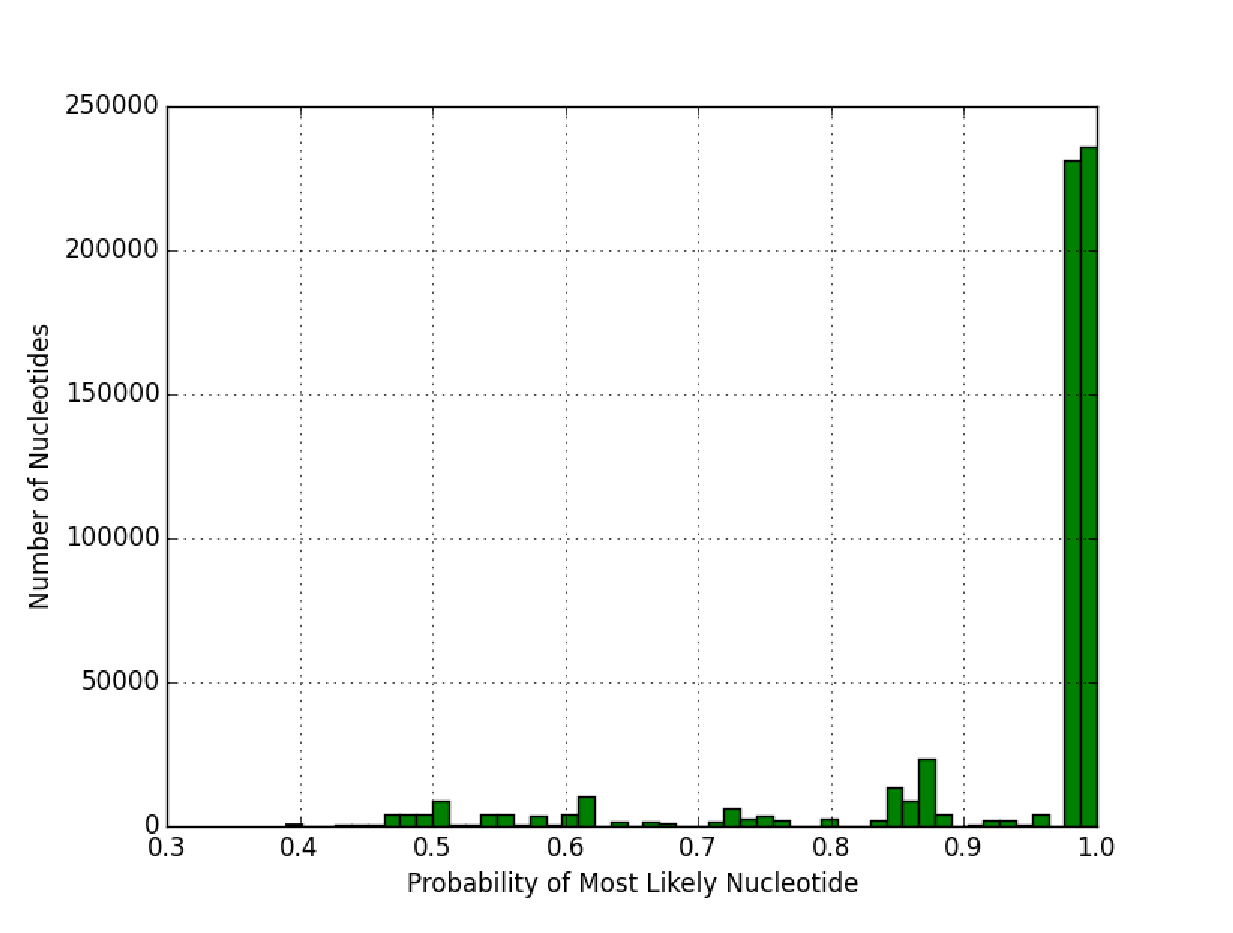
\includegraphics[scale=0.4]{data}
    \caption{Histogram of the frequencies that most-likely nucleotide appears at in the genome.}
    \label{data}
\end{figure}

For the following results, we used a probabilistic genome of length 604466 nucleotides. The probabilities in the genome are distributed with the majority of the mass being assigned to a single nucleotide and the remainder split equally between the three other nucleotides. As we can see from figure \ref{data}, the most frequent nucleotide at each genome is generally greater than 90\%, although this is not always the case.

\begin{table*}[]
\centering
\caption{Precision / Recall for \textbf{Maximum Likelihood Index}}
\label{ml}
\begin{tabular}{ll|llll}
\cline{3-6}
                                                       &              & \multicolumn{4}{l|}{\textbf{Threshold (as fraction of test query size)}}                                                                          \\ \cline{3-6} 
\textbf{}                                              &              & \multicolumn{1}{l|}{\textbf{0.25}} & \multicolumn{1}{l|}{\textbf{0.50}} & \multicolumn{1}{l|}{\textbf{0.75}} & \multicolumn{1}{l|}{\textbf{1.00}} \\ \hline
\multicolumn{1}{|l|}{\multirow{3}{*}{\textbf{Test Query Size}}} & \textbf{25}  & 0.23 / 0.80                         & 0.26 / 0.80                         & 0.43 / 0.80                        & 0.64 / 0.79                        \\ \cline{2-2}
\multicolumn{1}{|l|}{}                                 & \textbf{50}  & 0.18 / 0.89                        & 0.57 / 0.88                         & 0.78 / 0.86                         & 0.79 / 0.82                        \\ \cline{2-2}
\multicolumn{1}{|l|}{}                                 & \textbf{100} & 0.51 / \textbf{0.93}                          & \emph{0.79 / 0.90}                      & \textbf{0.81} / 0.85                         & 0.78 / 0.79                          \\ \cline{1-2}
\end{tabular}
\end{table*}

\begin{table*}[]
\centering
\caption{Precision / Recall for \textbf{Threshold of 0.925}}
\label{t925}
\begin{tabular}{ll|llll}
\cline{3-6}
                                                       &              & \multicolumn{4}{l|}{\textbf{Threshold (as fraction of test query size)}}                                                                          \\ \cline{3-6} 
\textbf{}                                              &              & \multicolumn{1}{l|}{\textbf{0.25}} & \multicolumn{1}{l|}{\textbf{0.50}} & \multicolumn{1}{l|}{\textbf{0.75}} & \multicolumn{1}{l|}{\textbf{1.00}} \\ \hline
\multicolumn{1}{|l|}{\multirow{3}{*}{\textbf{Test Query Size}}} & \textbf{25}  & 0.28 / 0.70                         & 0.30 / 0.70                         & 0.42 / 0.70                        & 0.58 / 0.69                        \\ \cline{2-2}
\multicolumn{1}{|l|}{}                                 & \textbf{50}  & 0.23 / 0.82                        & 0.58 / 0.81                         & 0.74 / 0.79                         & 0.74 / 0.76                        \\ \cline{2-2}
\multicolumn{1}{|l|}{}                                 & \textbf{100} & 0.56 / \textbf{0.89}                          & \emph{0.77 / 0.86}                    & \textbf{0.78} / 0.82                         & 0.75 / 0.76                          \\ \cline{1-2}
\end{tabular}
\end{table*}

\begin{table*}[]
\centering
\caption{Precision / Recall for \textbf{Threshold of 0.95}}
\label{t95}
\begin{tabular}{ll|llll}
\cline{3-6}
                                                       &              & \multicolumn{4}{l|}{\textbf{Threshold (as fraction of test query size)}}                                                                          \\ \cline{3-6} 
\textbf{}                                              &              & \multicolumn{1}{l|}{\textbf{0.25}} & \multicolumn{1}{l|}{\textbf{0.50}} & \multicolumn{1}{l|}{\textbf{0.75}} & \multicolumn{1}{l|}{\textbf{1.00}} \\ \hline
\multicolumn{1}{|l|}{\multirow{3}{*}{\textbf{Test Query Size}}} & \textbf{25}  & 0.29 / 0.62                        & 0.31 / 0.62                         & 0.41/ 0.62                       & 0.53 / 0.61                       \\ \cline{2-2}
\multicolumn{1}{|l|}{}                                 & \textbf{50}  & 0.27 / 0.77                        & 0.57 / 0.76                         & 0.69 / 0.74                         & 0.69 / 0.71                        \\ \cline{2-2}
\multicolumn{1}{|l|}{}                                 & \textbf{100} & 0.59 / \textbf{0.87}                          & \emph{0.76 / 0.85}                    & \textbf{0.77} / 0.81                         & 0.74 / 0.75                         \\ \cline{1-2}
\end{tabular}
\end{table*}


\begin{table*}[]
\centering
\caption{Precision / Recall for \textbf{Threshold of 0.975}}
\label{t975}
\begin{tabular}{ll|llll}
\cline{3-6}
                                                       &              & \multicolumn{4}{l|}{\textbf{Threshold (as fraction of test query size)}}                                                                          \\ \cline{3-6} 
\textbf{}                                              &              & \multicolumn{1}{l|}{\textbf{0.25}} & \multicolumn{1}{l|}{\textbf{0.50}} & \multicolumn{1}{l|}{\textbf{0.75}} & \multicolumn{1}{l|}{\textbf{1.00}} \\ \hline
\multicolumn{1}{|l|}{\multirow{3}{*}{\textbf{Test Query Size}}} & \textbf{25}  & 0.27 / 0.47                        & 0.28 / 0.47                         & 0.36/ 0.47                       & 0.42 / 0.47                      \\ \cline{2-2}
\multicolumn{1}{|l|}{}                                 & \textbf{50}  & 0.29 / 0.64                        & 0.52 / 0.63                         & 0.58 / 0.62                         & 0.58 / 0.60                        \\ \cline{2-2}
\multicolumn{1}{|l|}{}                                 & \textbf{100} & 0.58 / \textbf{0.79}                          & \emph{0.69 / 0.73}                    & \textbf{0.70} / 0.73                         & 0.67 / 0.68                        \\ \cline{1-2}
\end{tabular}
\end{table*}

We present the precision and recall for changing $T$ using various indexing schemes and test sequence lengths. Evaluation proceeded as described above.

\begin{figure*}
    \centering
    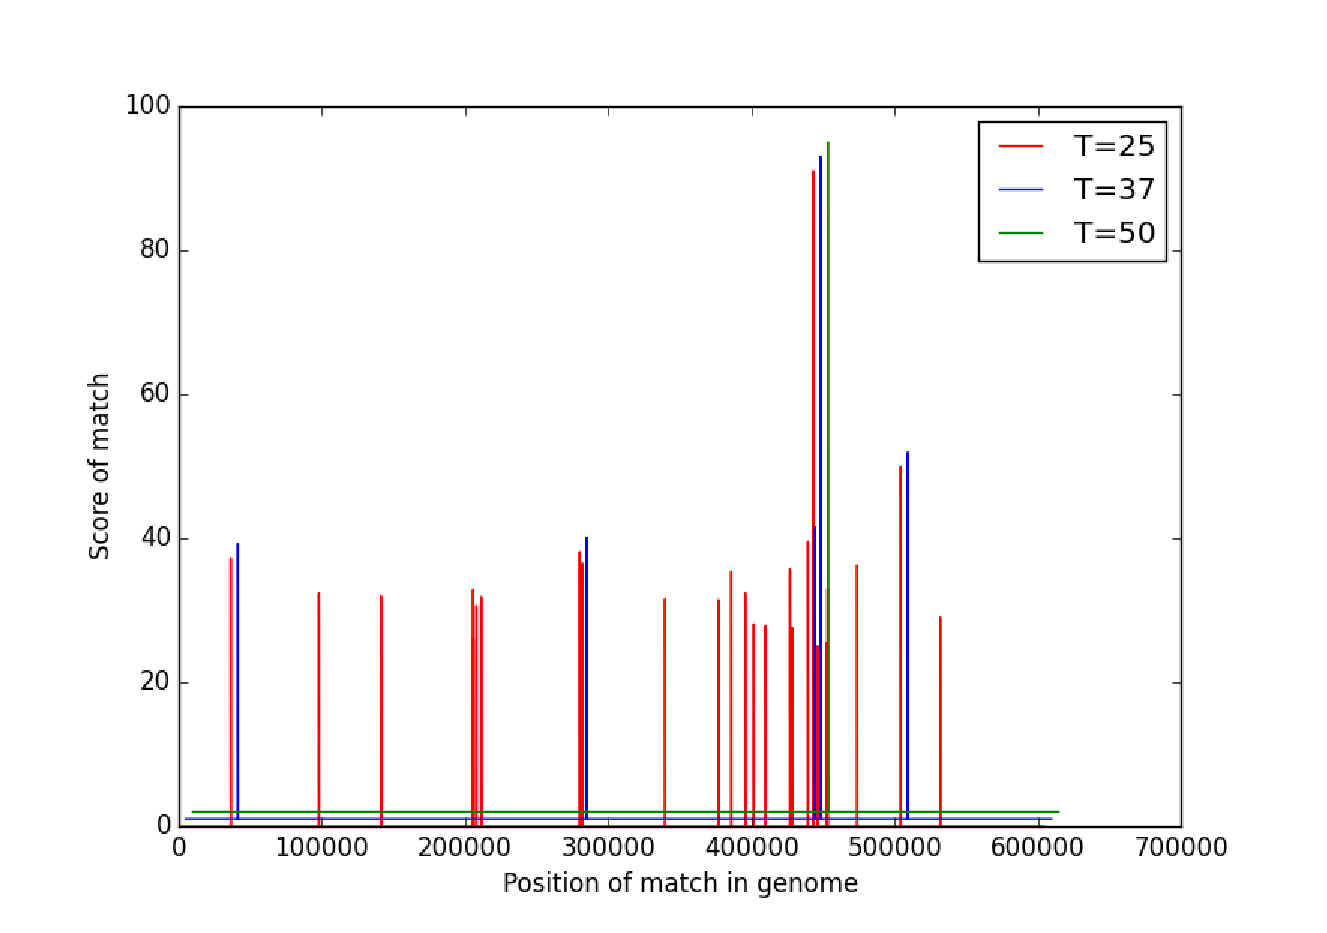
\includegraphics[scale=0.4]{dists}
    \caption{Scores of matches for a chosen test sequence of length 50 and their locations in the probabilistic genome. The gold standard shows where this sequence was actually generated from.}
    \label{dists}
\end{figure*}

Tables \ref{ml}, \ref{t925}, \ref{t95} and \ref{t975} present the precision and recall of each of our method. They are separated by index and show how changing the query sequence length and ungapped extension phase threshold affects the performance of our algorithm. In bold we can see the maximum precision and recall for each index, while what we evaluate to be the best threshold is in italic.

Figure \ref{dists} shows how changing the threshold affects the number of matches we return for a single test example. We can see that all thresholds are able to detect the match where the query sequence was generated from. However, lower thresholds return many more sequences with lower scores as well.

\section{Discussion}

\subsection{Choice of index}

As we can see in the tables \ref{ml}, \ref{t925}, \ref{t95} and \ref{t975}, the maximum likelihood index consistently outperforms the index with thresholds. It also turns out that the higher the threshold $t$, the weaker the performance gets. We suspect that high thresholds make it less likely that the index where the query was generated will become a seed during ProbaBLAST. Max-likelihood will consider lower probability nucleotides as long they are still the dominant nucleotide at their position.

\subsection{Selecting the best threshold values}

We experimented with various threshold sizes. Namely for each possible test sequence length, we considered thresholds of various fractions of the test sequence length ($\frac{1}{4}$, $\frac{1}{2}$, $\frac{3}{4}$, and $1$). We considered fractions so the number of matches wouldn't be as biased by the test string length. For example, a query string of length 25 would not have any ungapped matched of size 50. More dependencies on the size of the test sequence will be discussed in the next subsection.

It is common in all test sizes and indices (see tables \ref{ml}, \ref{t925}, \ref{t95} and \ref{t975}) that increasing the threshold will cause the precision to increase and the recall to decrease. 
This makes sense because as the threshold increases, we become more stringent about the score of a sequence to consider it a match. Thus only very high scoring pairs (usually matching to the generation location) are actually returned. This causes a higher precision as we are only returning relevant matches.

On the other hand, as we increase $T$, we are also less likely to include the actual generation location as a match due to mutations. When we don't return it as a match, the recall decreases. 

Thus tuning $T$ can affect the sensitivity of ProbaBLAST and it should be chosen based on the use case. If you only care about the highest scoring sequence, choosing a high $T$ will suffice (and it indeed what we evaluate for). But if you want anything that somewhat resembles the query sequence, you should choose a lower $T$. 

One interpretation of this (resulting from the new scoring scheme) is that a higher $T$ will force the algorithm to behave more like deterministic BLAST and only return high probability matches. Lower $T$'s allow for lower scoring nucleotides to enter the matches.

\subsection{Length of test sequences}
As mentioned earlier, we chose the size of the seed to be 11. In every table we can see that the length of the test sequence greatly affects the algorithm's performance. Indeed, the greater the length, the higher the precision and recall. We attribute this result to two facts:
\begin{enumerate}
\item The longer the sequence, the higher the chances that it is closer to the true distribution of the genome, making it more likely that there will be an alignment between part of the query and a seed in the site where the query was generated.
\item More importantly, longer sequences are less likely to randomly occur elsewhere in the genome. We can then distinguish between the true site where the query was generated and the ones that are similar to the true site.
\end{enumerate}


\subsection{Mutations}
We would like to provide some base intuition behind how mutations affect ProbaBLAST. 
ProbaBLAST is more robust to substitutions than indels because a substitution is less defined with this framework. It is hard for us to detect if a nucleotide at a given position differs from the most likely nucleotide because of the nature of the probabilistic genome or from a true substitution. Thus we can treat these simply as appearing with its respective frequency (the rest of the sequence is not affected). 

Indels are harder to correct for and we describe a method to handle this in future work. Lower thresholds could help account for this (at the expense of adding more matches) but a more robust method is described in Future Work. 

\begin{figure}
    \centering
    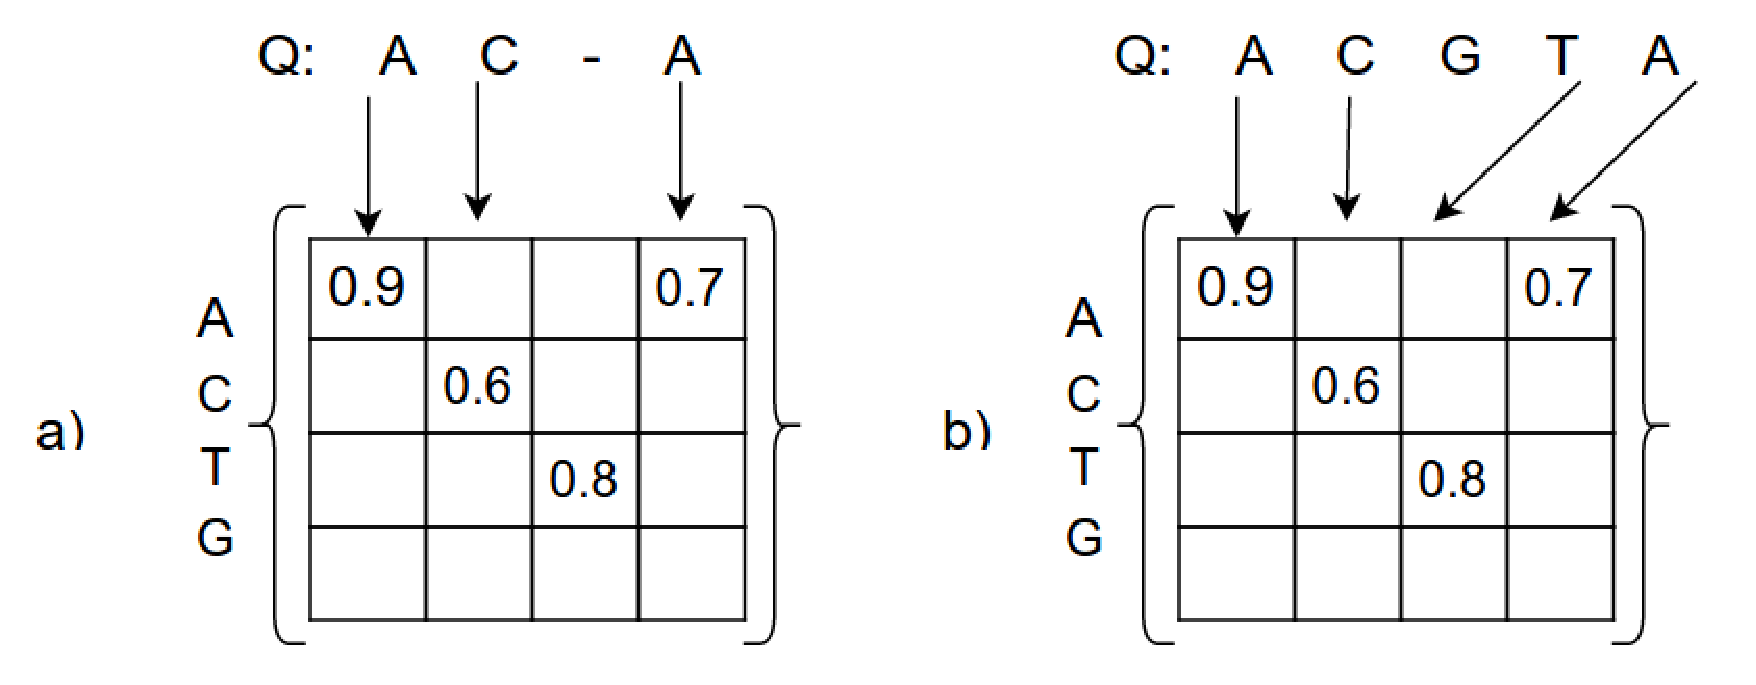
\includegraphics[scale=0.25]{indel}
    \caption{Proper alignment between $Q$ and $D$ showing a deletion (a) and an insertion (b).}
    \label{indel}
\end{figure}

\section{Conclusion}
In this paper, we described ProbaBLAST, a spin-off of BLAST that allows a user to match query sequences against a probabilistic genome (or database). It does this by finding seeds with high probability and then using a modified scoring metric during the ungapped phase. 

We showed that with the appropriate choices of $T$, ProbaBLAST can achieve high precision and recall scores on identifying matches with query sequences generated from the probabilistic genome then mutated.

\subsection{Future Work}

As we mentioned before, we did not investigate the gapped extension phase in depth. We now discuss how ProbaBLAST could be modified to allow our previously ungapped alignments to include gaps. We have a slightly different question than in BLAST but we claim that the Needleman-Wunsh algorithm can still be used to find the optimal alignment under a given scoring scheme - in this case our probabilistic scheme.

Before discussing this claim in detail, it is useful to first consider what an insertion or deletion means from a probabilistic genome. For the sake of this explanation, we assume $Q$ was generated by some unknown process from $D$. If we have an insertion into $Q$ then this new nucleotide would not be represented in $D$. Thus all nucleotides coming after the insertion will now point to the previous column of $D$ (see figure \ref{indel}b - shifts the distributions to the left). For a deletion in $Q$, a column of $D$ will now effectively never generate a nucleotide that is realized in $Q$. Thus all nucleotides coming after this deletion should be generated from the successor column in $D$ (see figure \ref{indel}a - shifts the distributions to the right). We can now view \"gaps\" as a device that shifts our distributions to try to best represent how the query sequence was generated.

Now instead of aligning a sequence to another sequence, we are aligning a deterministic sequence to a probabilistic sequence. Another way to phrase this is \"using the given scoring scheme, find the alignment that is most likely to have generated the query sequence.\" Let us consider the Needleman-Wunsch algorithm and provide an interpretation that holds for this problem. In the dynamic programming matrix X, on one dimension we have the nucleotides forming $Q$ (indexed by j), and along the other we have positions of $P$ (indexed by i). We get the following update equations:

\begin{equation}
X = max
\begin{cases}
X(i-1,j-1) + M(i,j) (a)\\
X(i-1, j) + c (b)\\
X(i, j-1) + c (c)
\end{cases}
\end{equation}

When we calculate scores we can interpret each part of the equations as follows:

\begin{description}
  \item[a)] Assume $q_j$ was generated from position $i$ of $P$.
  \item[b)] A deletion meaning position $i$ of $P$ never generated a realized nucleotide.
  \item[c)] An insertion meaning position $i$ has does not generate at this step (but may in the future).
\end{description}

The scoring scheme specifies that gaps should be allowed if it increases the likelihood of $Q$ by changing the positions nucleotides originated from.

\begin{thebibliography}{9}

\bibitem{originalBLAST}
Altschul, S.F., Gish, W., Miller, W., Myers, E.W., Lipman, D.J. 
\emph{Basic local alignment search tool. }
Journal of Molecular Biology 215(3), 403–410 (1990).

\bibitem{blast2}
Ma J., Zhang L.
\emph{Modern BLAST Programs}
Problem Solving Handbook for Comput Biol. and Bioinformatics, pp.3-19, Springer, 2010.


\end{thebibliography}

\end{document}